\documentclass[UTF8]{ctexart}
\usepackage{graphicx}
\usepackage{float}
\usepackage{subfigure}
\usepackage{amsmath}
\usepackage{graphicx}
\usepackage{geometry}
\usepackage{caption}
\geometry{left=2.0cm,right=2.0cm,top=2.54cm,bottom=2.54cm}
\linespread{1.5}
\makeindex
\bibliography{plain}
\title{ToF 传感器介绍}
\author{王澳917103860529\thanks{E-mail:877586493@qq.com}}
\date{\today}
\begin{document}
	
\maketitle

\section{ToF简介}
\subsection{定义}
\paragraph{维基百科}
时间飞行相机(TOF相机)是一个范围成像,其使用摄像系统时间飞行技术的照相机和用于图像的每个点对象之间的决心的距离,通过测量人工的往返时间由激光或LED提供的光信号。基于激光的飞行时间照相机是更广泛的无扫描器LIDAR类别的一部分,在该类别中,整个场景是由每个激光脉冲捕获的,而不是像在扫描LIDAR系统中那样逐点地捕获激光。民用飞行时间相机产品在2000年左右开始出现,[2]因为半导体工艺使这种器件的生产速度足够快。该系统覆盖范围从几厘米到几公里。的距离分辨率是大约1厘米。与标准2D摄像机相比,飞行时间摄像机的空间分辨率通常较低,截至2011年,大多数商用设备的像素分辨率为320×240像素或更小。与在其他用于捕获3D图像的3D激光扫描方法中,TOF相机每秒可提供多达160次操作,因此操作速度更快。
\paragraph{应用的广泛性}
\subsection{ToF技术和结构光技术的差别}
结构光 (Structured Light),指通过红外激光器,将具有一定结构特征的光线投射到被拍摄物体上,再由专门的红外摄像头进行采集反射的结构光图案,根据三角测量原理进行深度信息的计算。
\\
\\ iPhoneX上的Truedepth相机,用的是以色列PrimeSense公司的Light Coding技术。这种结构光方案,通过投射人眼不可见的伪随机散斑红外光点到物体上,每个伪随机散斑光点和它周围一定范围内的点集在空间分布中的每个位置都是唯一的,并将预先进行了存储。
\begin{figure}
	\centering
	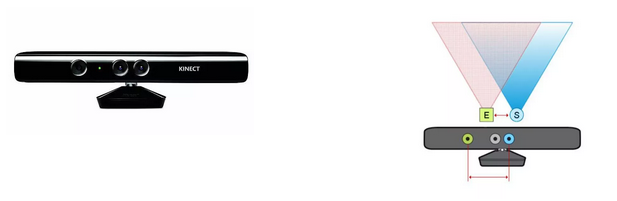
\includegraphics[width=0.7\textwidth]{ToFAND3D.png}
	\caption{3D结构光和ToF的区别}
	\label{Fig.main1}
\end{figure}
\\
这些散斑投影在被观察物体上的大小和形状根据物体和相机的距离和方向而不同,由此计算深度信息。这种方案和ToF相比计算量少功耗低,在近距离范围内精度更高,所以在人脸识别,和手势识别极具优势。
\begin{figure}
	\centering
	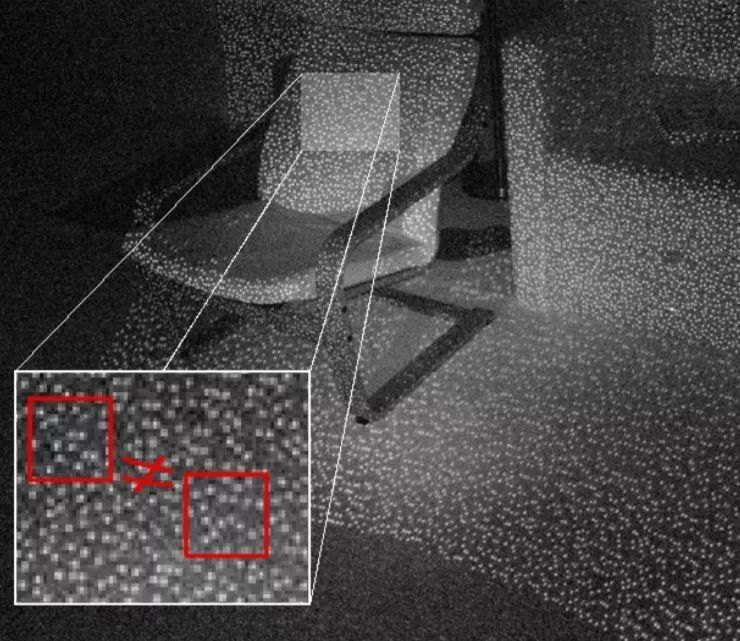
\includegraphics[width=0.7\textwidth]{3Dsensor.jpg}
	\caption{3D结构光点阵投影}
	\label{Fig.main1}
\end{figure}
说回ToF技术。相较之下,ToF设备要求发光器件与接收器件间尽可能接近,越接近,由于发射-接收路径不同所产生的误差就越小。因此,ToF技术更利于设备的小型化,对于手机或是AR产品实现轻便紧凑的外形非常重要。\\ 
测量距离方面,ToF也具备一定优势。由于ToF接收传感器所接收的每个像素点对应一个物体表面的实际位置,只要有反射光回来,就可以通过解相位的方法获取到深度。其测量精度不会随着测量距离的增大而降低,其测量误差在整个测量范围内基本上是固定的。而且由于太阳光并未经过调制,可以简单认为它对相位是没有影响的,所以ToF对于室外强光环境也有一定的鲁棒性。\\
分辨率方面,采用ToF技术的深度相机分辨率目前还偏低,一般也就320*240的水准,功耗上也略微不尽人意。   开发周期和解决方案方面,ToF因基于它的解决方案出现较晚,开发群体较为薄弱。而结构光技术,一方面PrimeSense(Kinect 1)当年的如日中天留下了无数成型的解决方案,有Intel支持的RealSense又有着非常强大的SDK,这些都使得基于结构光的开发周期可以比较短。\\   
综合来看,对于AR眼镜,无论是设备小型化需要还是实现SLAM需要的实时三维建图,ToF都有很大的优势。目前的一些“旗舰”产品HoloLens、Magic Leap One的深度摄像头用的也都是ToF技术。
\section{ToF工作原理}
\subsection{ToF相机组成单元}
\begin{enumerate}
	\item 照射单元\\
	照射单元需要对光源进行脉冲调制之后再进行发射,调制的光脉冲频率可以高达100MHz。因此,在图像拍摄过程中,光源会打开和关闭几千次。各个光脉冲只有几纳秒的时长。相机的曝光时间参数决定了每次成像的脉冲数。\\ 	
	要实现精确测量,必须精确地控制光脉冲,使其具有完全相同的持续时间、上升时间和下降时间。因为即使很小的只是一纳秒的偏差即可产生高达15cm的距离测量误差。\\
	 如此高的调制频率和精度只有采用精良的LED或激光二极管才能实现。\\
	一般照射光源都是采用人眼不可见的红外光源。
	\item 光学透镜\\
	用于汇聚反射光线,在光学传感器上成像。不过与普通光学镜头不同的是这里需要加一个带通滤光片来保证只有与照明光源波长相同的光才能进入。这样做的目的是抑制非相干光源减少噪声,同时防止感光传感器因外部光线干扰而过度曝光。
	\item 成像传感器 \\
	TOF的相机的核心。该传感器结构与普通图像传感器类似,但比图像传感器更复杂,它包含2个或者更多快门,用来在不同时间采样反射光线。因此,TOF芯片像素比一般图像传感器像素尺寸要大得多,一般100um左右。
	\item 控制单元 \\
	相机的电子控制单元触发的光脉冲序列与芯片电子快门的开/闭精确同步。它对传感器电荷执行读出和转换,并将它们引导至分析单元和数据接口。\\
	\item 计算单元 \\
	距离。为了得到更好的效果,通常会进行数据校准。	
\end{enumerate}
\subsection{工作原理}
\subsubsection{旅行时间原理}
在图像的顶部,您可以看到第一种方法,该方法是发送脉冲并测量时间间隔,直到它们在反射后返回为止\\
图像的中间显示了第二种方法,其中您可以调制光源的振幅并记录反射波的相移。\\
图像的底部代表第三种方法,该方法传输占空比为50%的方波,并记录在特定间隔内到达的返回光量。\\
\begin{figure}
	\centering
	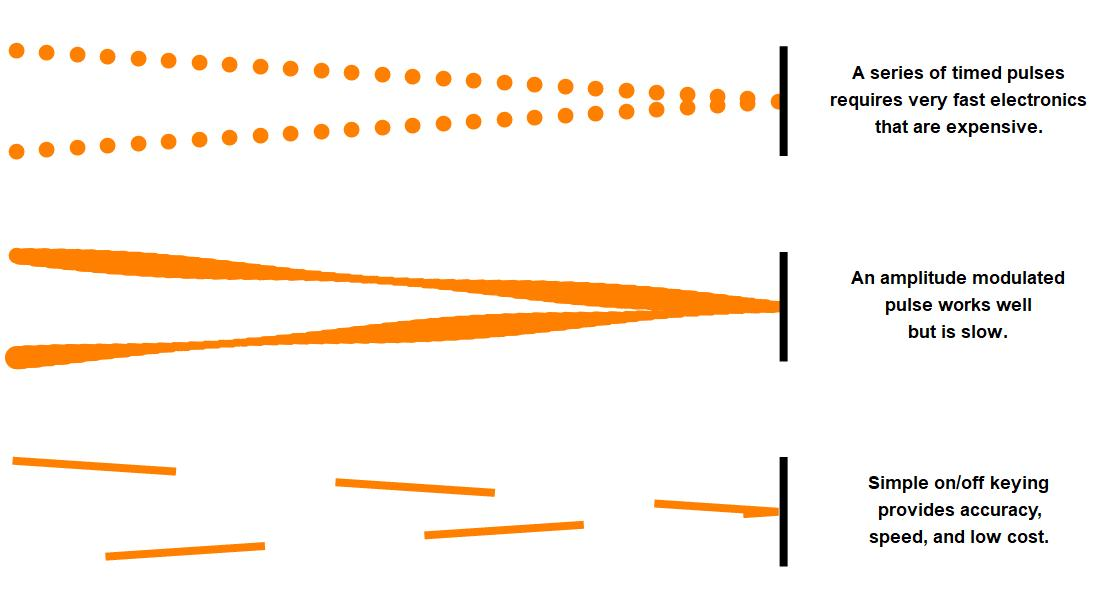
\includegraphics[width=0.9\textwidth]{principle.png}
	\caption{"工作原理"}
\end{figure}
\subsubsection{通过调幅波的相移确定距离}
通过相移和相角的作用,可以准确确定反射物体与传感器/接受器之间的距离
\begin{figure}
	\centering
	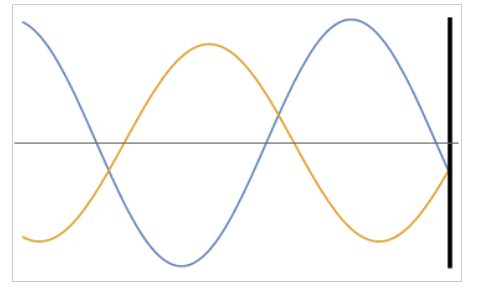
\includegraphics[width=0.8\textwidth]{相移.png}
	\caption{相移}
\end{figure}
如何快速测量正弦波的相位角?这涉及在四个等距的点(即90°或1/4$\lambda$的间隔)处测量接收信号的幅度
$$\varphi=arctan(\frac{A_1-A_3}{A_2-A_4}$$
\begin{figure}
	\centering
	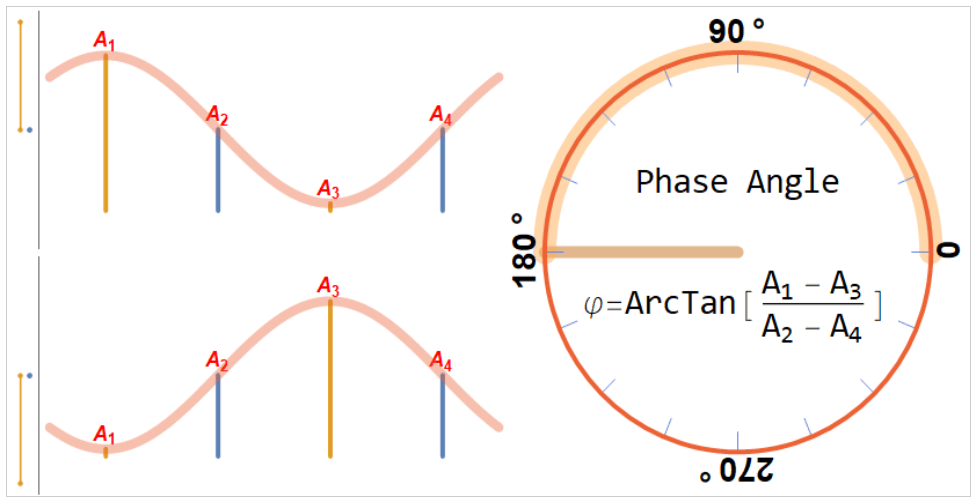
\includegraphics[width=0.8\textwidth]{原理插图.png}
	\caption{原理插图}
\end{figure}
\subsubsection{确定给定距离的工作频率}
$$d=\frac{C*\varphi}{4\pi F}$$
其中C是光速,$ \varphi$为相角以弧度为单位,$f$为调制频率
\subsubsection{通过带电电容器的差分电压测量确定相移}
下一个测量情况涉及频闪光源和每个像素有两个电容器的CMOS成像传感器。\\
时钟源产生占空比为50%的方波,并且该方波控制明亮的选通光源以及与每个像素内部的电荷存储电容器的连接。\\
下图显示了这种系统的示例:
\begin{figure}
	\centering
	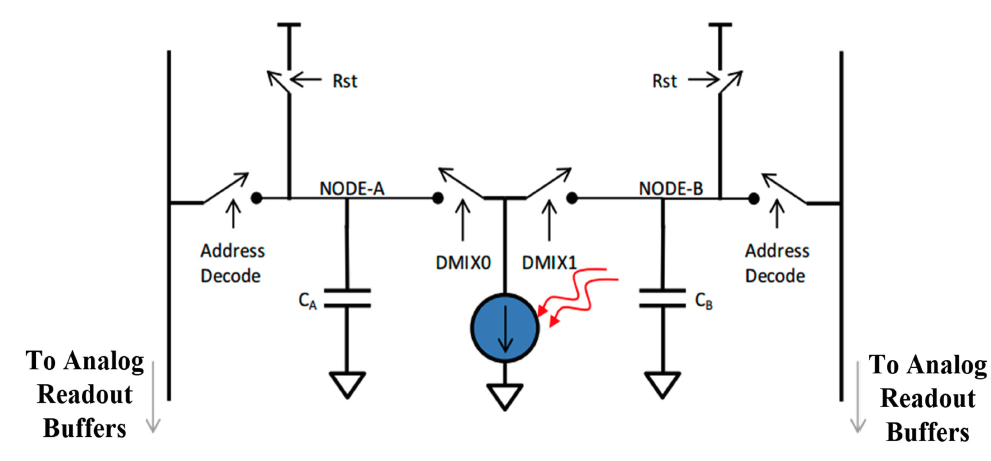
\includegraphics[width=0.8\textwidth]{电路.png}
	\caption{“光子混合器设备固态阵列LiDARS的快速校准方法”中的图像显示了一个CMOS像素,其中两个电荷存储电容器交替连接以记录入射光。}
\end{figure}
光线离开光源,反射离开物体,然后撞击像素,在此处像素将作为电荷被记录在上方的电容器C A或C B中。电容器使用相同的时钟源以与照明源相同的频率交替连接至像素。  \\
这种巧妙的安排意味着电容器中的差分电荷直接与相位偏移有关。而相位则取决于波长以及到目标和目标之间的距离。\\
\begin{figure}
	\centering
	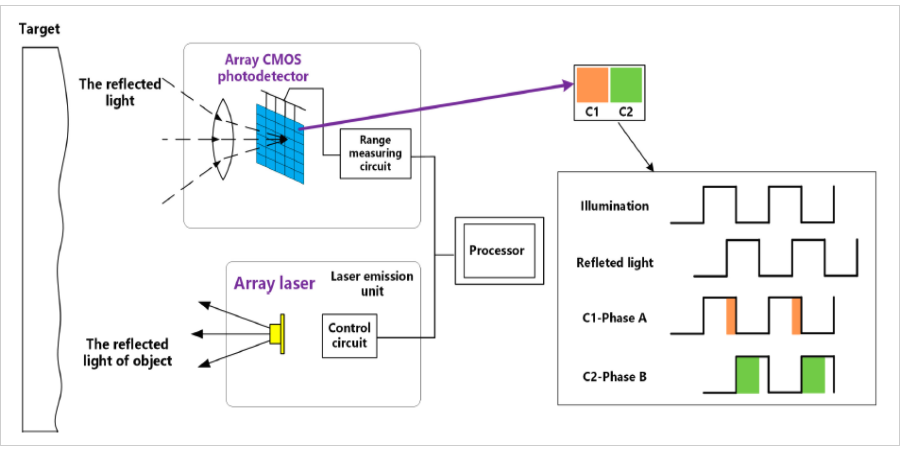
\includegraphics[width=0.8\textwidth]{快速校准方法.png}
	\caption{“光子混合器设备固态阵列LiDARS的快速校准方法”}
\end{figure}
可以照亮被摄对象充电容器所需的次数。只要距离恒定,充电比例将保持不变\\
\begin{figure} 
	\begin{minipage}[t]{0.5\linewidth} 
		\centering 
		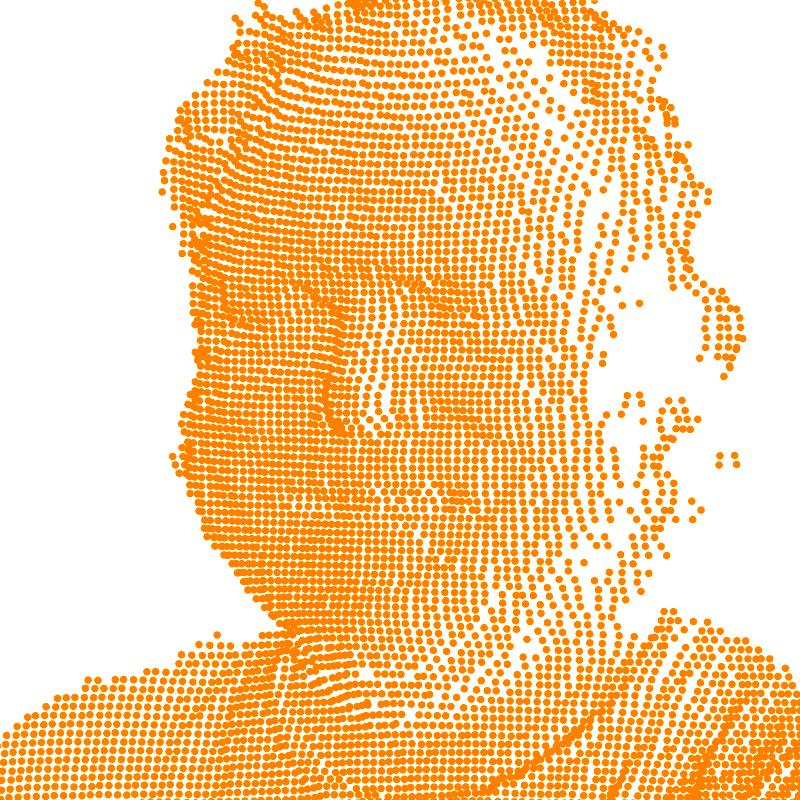
\includegraphics[width=2.0in]{深度数据.jpg} 
		\caption{深度数据} 

	\end{minipage}% 
	\begin{minipage}[t]{0.5\linewidth} 
		\centering 
		\includegraphics[width=1.8in]{深.png} 
		\caption{ToF镜头产生的图像} 

	\end{minipage} 
\end{figure}
\section{ToF镜头的广泛应用}
\begin{itemize}
	\item 消费者\\从AR(增强现实)和VR(虚拟现实)耳机到具有高级照相和安全功能的智能手机,ToF技术预计将成为下一代消费电子产品的重要组成部分。\\
	在AR / VR头戴式耳机中,ToF系统获取的深度信息从字面上为用户提供了现实的附加维度。在智能手机中,该技术将使相机能够开发出具有DSLR品质的摄影效果,实现更逼真的AR / VR功能,并提供防止不必要的外部访问的额外保护。
	\item 工业4.0\\
	智能传感器,特别是深度传感器的使用在制造以及运输和物流中越来越普遍。\\
	从用于质量检查的工业机器视觉到用于资产管理的体积检测,再到用于自动制造的导航,制造业正在采用这些传感技术,并朝着针对恶劣工业环境设计的高分辨率系统发展。
	\item 汽车行业\\
	在下一代汽车中,机舱中的ToF系统将能够监视驾驶员及其乘客的位置和状态,并在驾驶员丧失能力的情况下接管控制权并将汽车调至安全状\\态据说,通过ToF技术实现的手势控制系统是汽车的下一代用户界面,使驾驶员可以通过简单的手势来接听打来的电话,更改音频输入源,甚至调节气候控制。手或手指。
	\item 卫生保健\\
	鉴于最近的大流行,用于远程距离和深度测量的飞行时间技术在医疗保健中变得越来越重要。在各种环境中,通过手势进行的非接触式操作控制,婴儿呼吸的远程监视以及社交距离的监视只是可以使用ADI飞行时间技术的少数应用中的一些。
	\item 安全与监视\\
	与传统的2D图像传感技术相比,ADI的高分辨率深度传感技术具有明显的优势。高分辨率的深度使对人和物体的分类更加容易,并且置信度更高。从商业/零售进入/退出(用于安全和监视)到检测跌倒或伤害自己的人(用于医疗应用),这可以被用于许多应用用例中。
	\item 机器人技术\\
	高分辨率ToF系统对于使自主机器和机器人能够感知其环境并规划其路径以最佳,可靠和安全地完成其任务至关重要。此外,3D成像可以在人类和协作机器人共同工作的应用中启用安全功能。
\end{itemize}
\begin{figure*}[htbp]
	\centering
	
	\subfigure[]{
		\begin{minipage}[t]{0.33\linewidth}
			\centering
			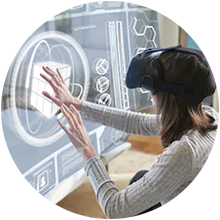
\includegraphics[width=1.651in]{1.png}\\
			\vspace{0.02cm}
			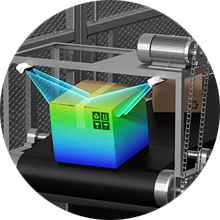
\includegraphics[width=1.651in]{2.png}\\
			\vspace{0.02cm}
			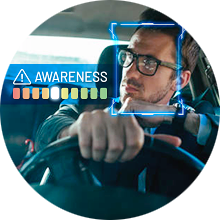
\includegraphics[width=1.651in]{3.png}\\
			\vspace{0.02cm}
			%\caption{fig1}
		\end{minipage}%
	}%
	\subfigure[]{
		\begin{minipage}[t]{0.33\linewidth}
			\centering
			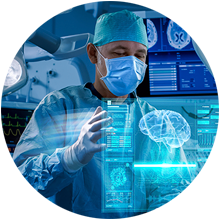
\includegraphics[width=1.651in]{4.png}\\
			\vspace{0.02cm}
			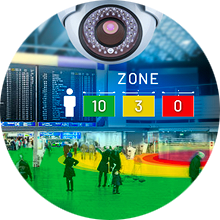
\includegraphics[width=1.651in]{5.png}\\
			\vspace{0.02cm}
			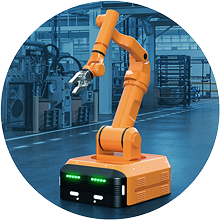
\includegraphics[width=1.651in]{6.png}\\
			\vspace{0.02cm}
			%\caption{fig1}
		\end{minipage}%
	}%
	
	
	\centering
	\caption{广泛的应用}
	\vspace{-0.2cm}
	\label{fig:compare_fig}
\end{figure*}
\section{产业现状}
2017年,iPhoneX的Face ID将结构光三维视觉的产业链整合起来,由于TOF的产业链与结构光比较一致,小型化的TOF三维视觉技术产业链也随之发展起来。TOF三维视觉产业链中主要包括TOF传感器芯片厂商、模组厂商、算法厂商及VCSEL、DOE等元器件厂商。其中VCSEL(Vertical Cavity Surface EmittinLaser)译为垂直腔面发射激光器,简称面射型激光,是TOF技术方案所采用的光源。EDO(Diffraction Optical Element)就是衍射光学元件,用来使发出的光保持均匀,准确测距。这两者都是TOF三维视觉硬件的核心元器件。\\
TOF技术对光学传感芯片要求高,而目前国外传感器芯片厂商在国内TOF产业链中占据着主导地位。国外芯片厂商通过模组厂商牵线搭桥与手机厂商签订单,成为目前在国内TOF三维视觉方案在手机上的落地的主要模式。有业内人士称,近来正是因为索尼、三星、英飞凌等大厂在往TOF芯片砸钱,进而推动了模组厂商提高相关的产能。例如索尼就在今年初宣布加大TOF投入,夏季将实现3D ToF图像传感器的量产。据了解,国内超过一半的手机TOF相机方案都是采用的索尼感光芯片。索尼2015年收购了长于TOF影像技术的Softkinetic公司,之后逐渐凭借手机摄像头市场已有的领先地位,在我国占据了远高于TOF鼻祖pmd的市场份额。除了索尼,ADI是国内被选择最多的芯片商之一。据了解,其TOF的感光芯片技术比较成熟,比如ADI早就研发出VGA(分辨率达到640x480dpi)感光芯片,只是近年随着3D应用的兴起才又将其从“箱底”启用。\\
不过,目前TOF传感器芯片在国内也有炬佑智能、歌尔等企业做的比较好。比如,炬佑智能公司自研了320x240dpi等多种分辨率的850nm和940nmToF传感芯片,已为扫地机器人、VR/AR、手机等应用提供完整的脉冲TOF方案,但是其VGA(分辨率达到640x480dpi)感光芯片仍在研发之中。在TOF相机模组的封装与测评方面,舜宇光学、欧菲光、威豪等国内厂商都凭借各自的垂直领域优势占据着龙头地位。舜宇光学具有镜头这一垂直领域优势,同时还拥有众多元器件的子公司。欧菲光旗下的VCSEL供应商纵慧也进入了华为手机TOF方案供应链,欧菲光和豪威分别由于在滤光技术及手机摄像头模组上的渠道优势在国内TOF市场中占据一定份额。\\
\begin{figure}
	\centering
	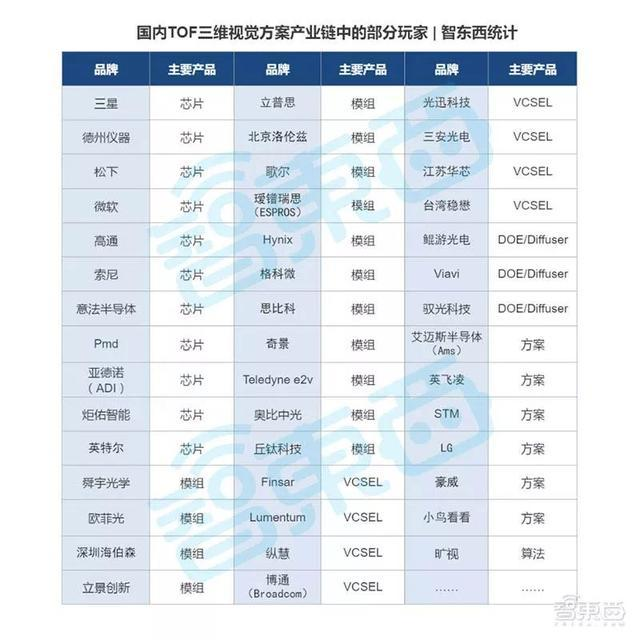
\includegraphics[width=0.8\textwidth]{产业现状.jpg}
	\caption{“产业现状”}
\end{figure}	
	

\end{document}
